% ============================================================
% Filtros Pasa-banda (Band-Pass)
% ============================================================
\section{Filtros Pasa-banda (Band-Pass)}

\subsection{Butterworth}

\begin{figure}[H]
	\centering
	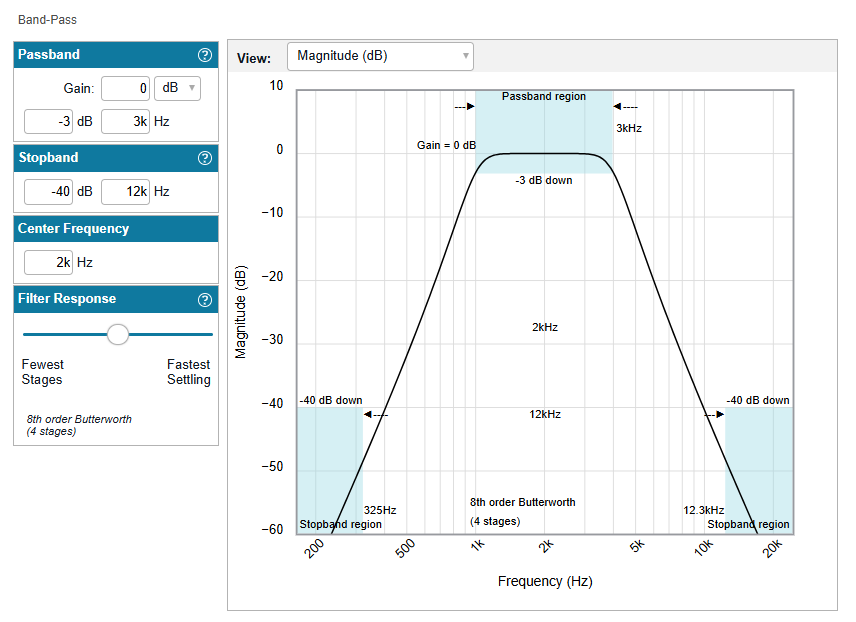
\includegraphics[width=0.9\textwidth]{img/bp_butterworth_respuesta.png}
	\caption{Respuesta en magnitud del filtro pasa-banda Butterworth de 8.\textsuperscript{o} orden (centrado en 2\,kHz).}
	\label{fig:bp_butterworth_respuesta}
\end{figure}

\begin{figure}[H]
	\centering
	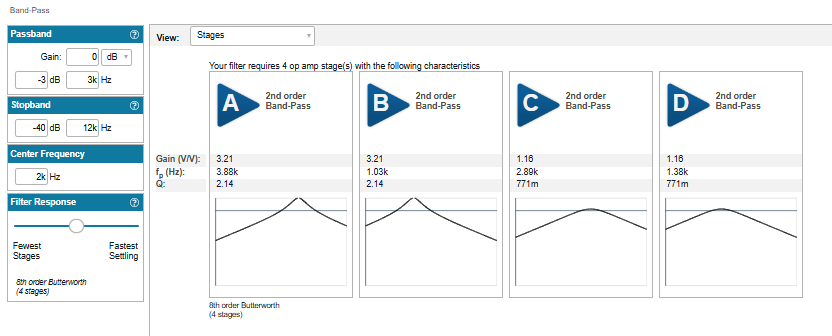
\includegraphics[width=0.9\textwidth]{img/bp_butterworth_etapas.png}
	\caption{Configuración de etapas (\textit{Stages}) del filtro pasa-banda Butterworth: cuatro etapas de segundo orden.}
	\label{fig:bp_butterworth_etapas}
\end{figure}

\begin{figure}[H]
	\centering
	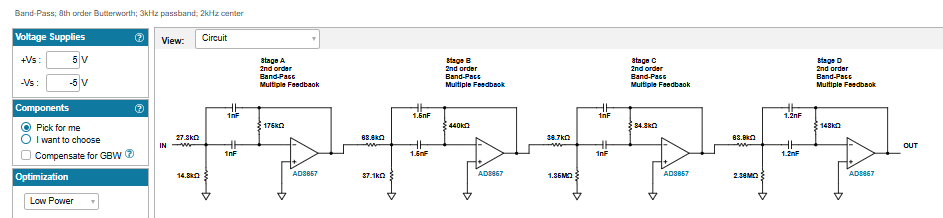
\includegraphics[width=\textwidth]{img/bp_butterworth_circuito.png}
	\caption{Circuito del filtro pasa-banda Butterworth.}
	\label{fig:bp_butterworth_circuito}
\end{figure}

% ------------------------------------------------------------
\subsection{Chebyshev}

\begin{figure}[H]
	\centering
	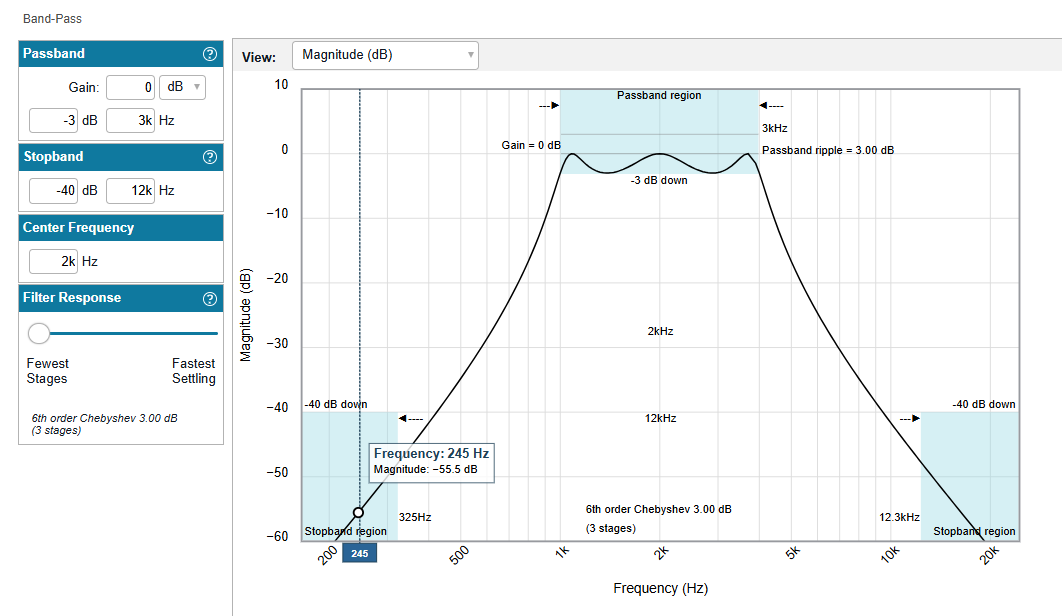
\includegraphics[width=0.9\textwidth]{img/bp_chebyshev_respuesta.png}
	\caption{Respuesta en magnitud del filtro pasa-banda Chebyshev de 6.\textsuperscript{o} orden (rizo de 3\,dB, centrado en 2\,kHz).}
	\label{fig:bp_chebyshev_respuesta}
\end{figure}

\begin{figure}[H]
	\centering
	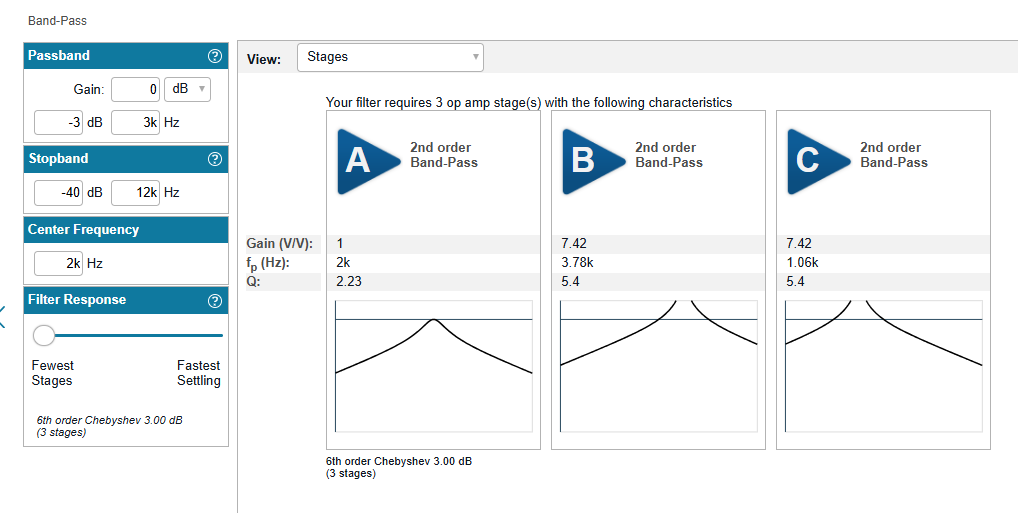
\includegraphics[width=0.9\textwidth]{img/bp_chebyshev_etapas.png}
	\caption{Configuración de etapas (\textit{Stages}) del filtro pasa-banda Chebyshev: tres etapas de segundo orden.}
	\label{fig:bp_chebyshev_etapas}
\end{figure}

\begin{figure}[H]
	\centering
	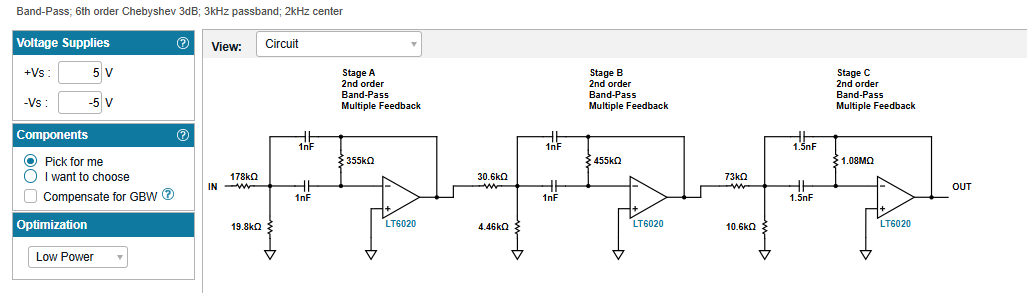
\includegraphics[width=\textwidth]{img/bp_chebyshev_circuito.png}
	\caption{Circuito del filtro pasa-banda Chebyshev.}
	\label{fig:bp_chebyshev_circuito}
\end{figure}

% ------------------------------------------------------------
\subsection{Bessel}

\begin{figure}[H]
	\centering
	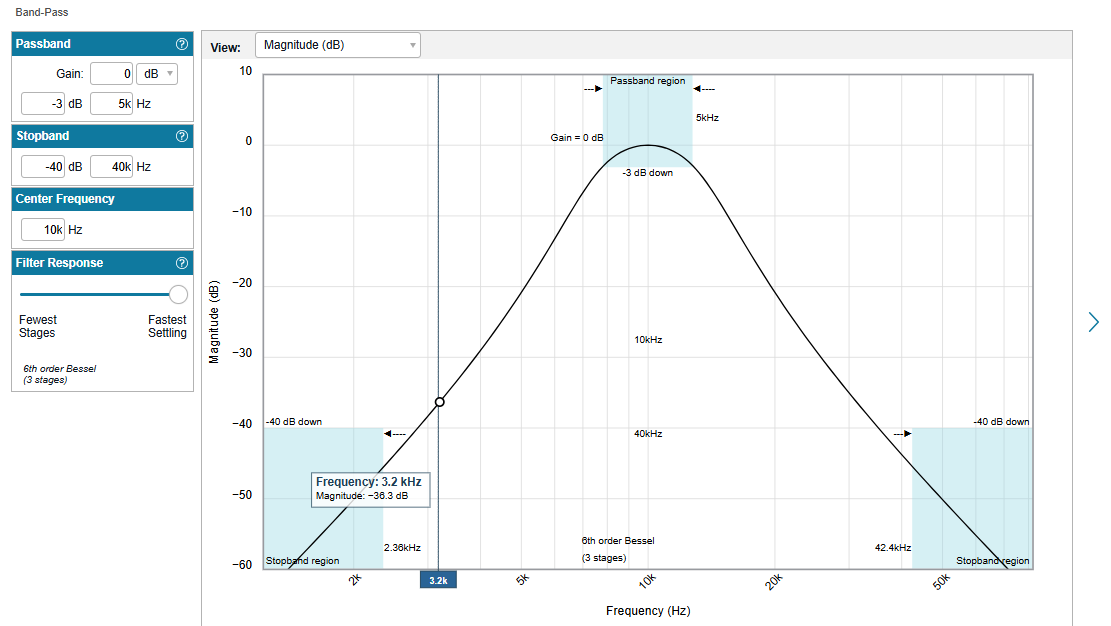
\includegraphics[width=0.9\textwidth]{img/bp_bessel_respuesta.png}
	\caption{Respuesta en magnitud del filtro pasa-banda Bessel de 6.\textsuperscript{o} orden (centrado en 10\,kHz).}
	\label{fig:bp_bessel_respuesta}
\end{figure}

\begin{figure}[H]
	\centering
	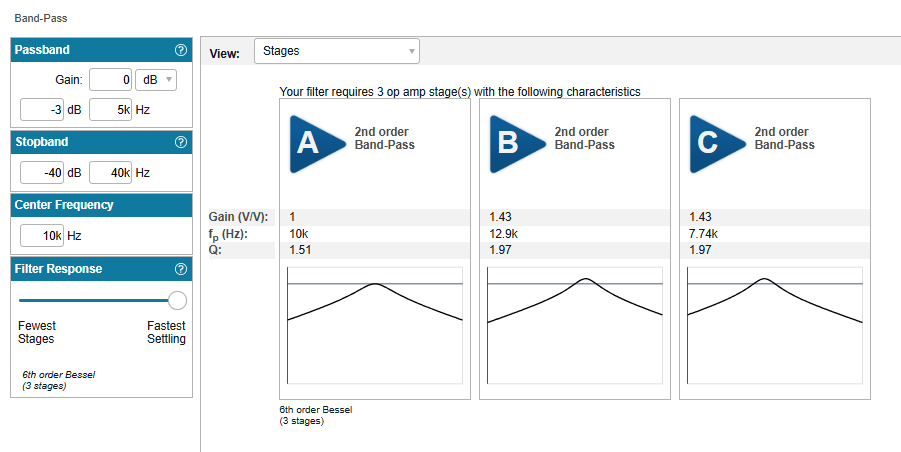
\includegraphics[width=0.9\textwidth]{img/bp_bessel_etapas.png}
	\caption{Configuración de etapas (\textit{Stages}) del filtro pasa-banda Bessel: tres etapas de segundo orden.}
	\label{fig:bp_bessel_etapas}
\end{figure}

\begin{figure}[H]
	\centering
	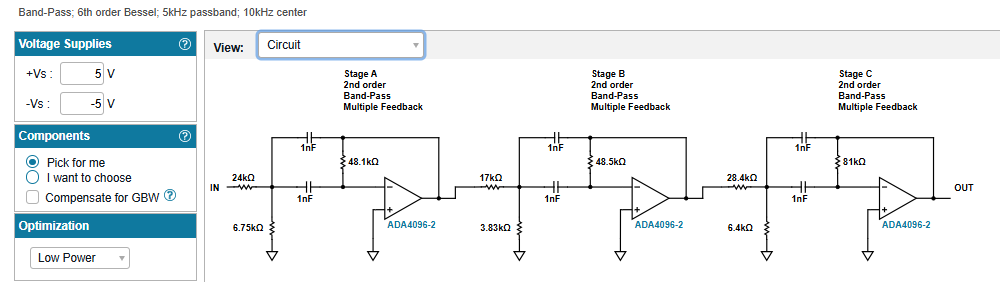
\includegraphics[width=\textwidth]{img/bp_bessel_circuito.png}
	\caption{Circuito del filtro pasa-banda Bessel.}
	\label{fig:bp_bessel_circuito}
\end{figure}
